\pagenumbering{arabic}
\setcounter{page}{1}
\pagestyle{fancy}
\chapter*{Introduction}
\markboth{Introduction}{Introduction}
\addcontentsline{toc}{chapter}{Introduction}
\label{chapter:introduction}

% FORMATTING
\pagenumbering{arabic}
\setcounter{page}{1}
\pagestyle{fancy}
% FORMATTING

Industrial automation is witnessing a paradigm shift from isolated robotic systems towards collaborative scenarios where humans and robots share a common workspace and physically interact. This recent field, known as \emph{physical human-robot interaction} (pHRI), presents a vision for the future of manufacturing, promising enhanced efficiency, flexibility, and safety. pHRI has the potential to bring new perspectives to various fields: human rehabilitation, sport training assistance, or medical and surgery assistance (\cite{benoussaadEditorialPhysicalHumanrobot2022}).

In today's manufacturing industry, robots play an essential role. 
Traditional industrial robots, operating within safety cages, are instrumental in automating repetitive, high-precision tasks. The worldwide supply of industrial robots increases annually: in 2022, almost 4 million industrial robot were operational, with more than 500,000 new units installed per year since 2021 (\cite{ifr2023}). Furthermore, small and medium-sized companies are drawn to the more available, affordable, compact, easy-to-use solutions which are \emph{collaborative robots}, or \emph{cobot}. These robots, specifically designed for human collaboration, focus on creating a smooth virtual or haptic interaction within a shared workspace (\cite{peshkinCobotArchitecture2001}; \cite{villaniSurveyHumanRobot2018}).

However, human presence in a collaborative process introduces challenges such as unpredictable behavior, fatigue, ergonomic considerations, and safety concerns. Consequently, realizing an ideal pHRI vision requires a deep understanding of the complexities inherent in human-robot collaboration, particularly the biomechanical and cognitive factors (\cite{camblorExploitationMouvementRobot2024}) that influence human behavior during physical interaction.

To enhance efficiency, collaborative physical interaction must leverage the unique capabilities of both humans and robots (\cite{colgateCobotsRobotsCollaboration1996}). Robots excel to achieve great force capacities, precision, repeatability, endurance, and speed. Humans, on the other hand, offer adaptability, the ability to handle uncertainty, and dexterity, particularly with their hands. To effectively leverage these complementary strengths, a clear understanding of both human and robot capabilities is thus crucial. Specifically, identifying the challenges faced by humans in collaborative tasks is essential for designing robots that can effectively assist them. This necessitates incorporating such knowledge into the robotic framework design. For example, control algorithms can enable cobots to adapt to human actions, ensuring smooth and seamless collaboration. 

This thesis focuses on considering the exertable forces of an individual to improve robotic assistance and ensure greater safety in collaborative scenarios with physical interaction at the hand. First, we will describe how such scenarios occur and the \emph{in vivo} and \emph{in silico} challenges of integrating these forces into the robotic framework. Then, we will consider how this thesis' chosen approach of representating maximal force exertions should reveal more about the biomechanical muscle properties of a human. Finally, the thesis outline will be presented with the main results found within this manuscript.

\section*{Shared force exertion in Human-Robot collaboration}
\addcontentsline{toc}{section}{Shared force exertion}
As robotic technologies continue to advance, with more cobots capable of adapting to increasingly dynamic scenarios where their behavior is optimized for collaborative performance (\cite{albertoPredictiveControlCollaborative2023}), there is an emergence of \emph{personalized cobots}, which are essentially cobots customized to an individual workers' physical needs, preference, and skill levels, leading to more personalized and effective collaboration.

When considering robots in dynamic environments, the concept of force becomes central. Cobots can be equipped with an array of sensors to detect external forces and torques applied to their structure. This allows them to react instantly to unexpected contact, adjusting their movements or stopping altogether to prevent collisions and ensure human safety. Advanced force control algorithms enable cobots to perform tasks requiring precise force regulation, such as assembly operations or collaborative manipulation (\cite{bicchiPhysicalHumanrobotInteraction2008}). However, in a more collaborative industrial framework where human safety is a primal concern, it is essential to \emph{express} the force limits exertable by the human so the robot can account for them. Knowledge of these limits is thus required for safety, preventing the robot from applying excessive force and potentially injuring the human.

The forces exerted by a robot at its end-effector can be understood via a mathematical description of its (almost) rigid components linked by joints, and the forces applied to the joints. While other modeling tools exist, such as incorporating machine learning techniques to optimize robot motions (\cite{peternelAdaptationRobotPhysical2016}), rigid body modeling offers a key advantage: it clarifies how forces are transmitted between components. Therefore, applying this modeling approach to the human body is particularly relevant, for instance to evaluate how a physical workload can generate musculoskeletal disorders (\cite{hoozemansMechanicalLoadingLow2004}). These models, known as \emph{musculoskeletal models} when based on a human, provide a suitable framework for studying forces in both humans and robots. They involve the inclusion of \emph{muscles}, which are physiological components responsible for the generation of joint motion. Since muscle forces can be described as a mechanical system (\cite{hillHeatShorteningDynamic1938}), robotic modeling techniques can be applied to mathematically model muscles and analyze their role in movement generation.

Given that physical Human-Robot interaction often involves contact between the human hand and the robot's end-effector, an upper-limb musculoskeletal model is particularly relevant (\cite{holzbaurModelUpperExtremity2005}). However, an individual can exert force through various combinations of different muscles. This \emph{muscle redundancy} allows for different force exertion strategies. These combinations are modeled through activation patterns, which quantify how each muscle exerts force based on the specific movement and the activation of other muscles (\cite{zajacMuscleTendonProperties1989a}). Since there are a finite number of muscles in the upper-limb, the combination of their tensions necessarily produces a maximal force at the end-effector for a given posture and activation pattern.

The exerted force at the hand is therefore limited, with this limit depending on both the upper-limb posture and the direction of force application (\cite{oshimaRoboticAnalysesOutput2000}, \cite{hernandezIsometricForceCapabilities2015}). Measuring maximal forces during dynamic movements is challenging, as it requires participants to exert maximum effort throughout the movement, potentially leading to exhaustion and discomfort (\cite{roseFatigueRecoveryStatic2014}). Therefore, the focus is on measuring maximal \emph{isometric} forces, which are forces exerted in a fixed posture. In physical Human-Robot interaction, near-static scenarios occur when tasks require hand dexterity and precision, such as in manufacturing with small objects (\cite{javaidSignificantApplicationsCobots2022}). Focusing on isometric forces in such scenarios allows for more controlled experimental procedures. However, since maximal isometric force depends on the direction of exertion, measurements must be taken in multiple directions. Due to the lack of standardized protocols for selecting these directions, an arbitrary number are typically chosen, ensuring sufficient coverage of the 3D force space. Since muscle rest must be taken into account during experiments, this can result in rather long procedures for the participant. Therefore, this thesis first addresses the following challenge:

\begin{mdframed}
    \begin{center}
        \textbf{Challenge 1:} \\
        How can the measurement of maximal isometric forces be performed efficiently within a reasonably long experiment?
        % How can the measurement of maximal isometric forces be made more efficient and less time-consuming for participants?
    \end{center}
\end{mdframed}

Furthermore, the complexity of human upper limb models for \emph{in silico} computations can vary significantly depending on the context. Given the computational demands of musculoskeletal models, it is crucial to determine the appropriate level of model complexity. This includes deciding which muscles to include, as well as the level of detail in representing their paths around bones and joints. For instance in the force exertion context, it might not be useful to consider a 3-dimensional robot arm if the studied forces are only applied on a 2-dimensional plane (\cite{sasakiHigherDimensionalSpatial2010a}). Furthermore, the inter-individual variability in muscle physiology necessitates the development of \emph{personalized} musculoskeletal models. These models adapt a generic upper-limb model to reflect the specific physiology of an individual. Indeed, maximal isometric forces are influenced by various cognitive and physiological factors, including muscle geometry, bone structures, training, muscle fatigue, etc. Therefore, it is essential to determine the level of detail required to accurately characterize an individual's maximal force capabilities \emph{in silico}. As such, this thesis addresses this second scientific challenge:

\begin{mdframed}
    \begin{center}
        \textbf{Challenge 2:} \\
        How detailed and personalized must a musculoskeletal model of the human upper-limb be to accurately represent the exertable maximal isometric forces at the hand of an individual?
    \end{center}
\end{mdframed}

While the two challenges outlined above focus on practical applications required to either experimentally measure maximal isometric forces or represent them \emph{in silico}, the next section addresses a more fundamental question of how to represent these forces to gain deeper biomechanical insights.

\clearpage
\section*{Maximal isometric forces: is a set-theoretic approach suitable?}
\addcontentsline{toc}{section}{Maximal isometric forces: is a set-theoretic approach suitable?}
Sets provide a valuable tool in robotics, offering a compact and versatile framework for representing various robotic concepts, such as dynamic workspaces and 3D obstacles (\cite{barretteDeterminationDynamicWorkspace2005}; \cite{lauWrenchClosureWorkspaceGeneration2011}; \cite{scottConstrainedZonotopesNew2016}). Sets can be used to quantify and assess physical abilities, such as the manipulability index for robots (\cite{yoshikawaManipulabilityRoboticMechanisms1985}) and the robot carrying capacity index (\cite{skuricCoupledViewPhysical}), in both humans and robots. Essentially, sets offer a different perspective on a problem, enabling the use of a broader range of methods to derive meaningful insights.

This thesis explores maximal isometric forces through a set-theoretic lens. Instead of focusing on individual forces, we consider the a \emph{collection} of maximal isometric forces within a posture as a unified object of study. This approach presents both experimental and mathematical hurdles. Tools for analyzing these forces, especially those implemented numerically, are more efficient in regard to a \emph{locus} approach: examining single elements like points, vectors, or lines. However, modern mathematics, particularly since the mid-20th century, have increasingly relied on a set-theoretic foundation (\cite{bourbakiTheorieEnsembles2006}), where everything is considered a set. Analyzing collections of objects unlocks a deeper understanding of their interdependencies and how they behave in various contexts. In essence, a set-theoretic approach allows us to describe elements through their \emph{structured} interactions. However, this structure is not always immediately apparent. Even seemingly random sets possess structure, which can be revealed through concepts like probability distributions.

\begin{figure}[!htb]
    \captionsetup{justification=centering}
        \centering
        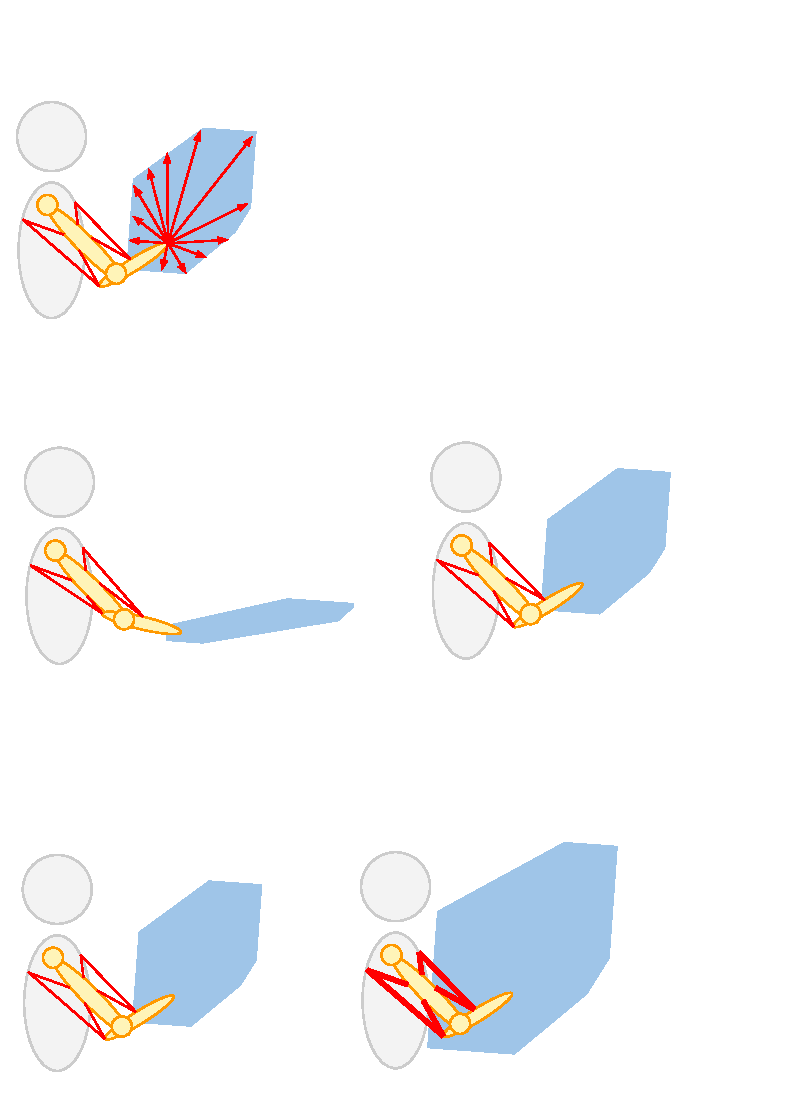
\includegraphics[trim={0 370 250 40},clip,width=0.3\linewidth]{img/chapter_1/ffs_characteristics.pdf}
    \caption{The \emph{force feasible set} of an individual in a specific posture denotes all maximally exertable forces in this upper-limb posture.}
    \label{fig:ffs_simple}
\end{figure}

Abstract mathematics emphasizes understanding how structures are preserved under transformations of their underlying elements. More interestingly, it also seeks to extract the original structure by analyzing the transformed elements. This approach is relevant for the study of maximal isometric forces. These forces, viewed as individual elements, are fundamentally derived from muscle activation patterns. A key goal of this thesis is to analyze the structure within these produced forces to gain insights into the collective behavior of muscle activations.

As such, the collection of all exertable maximal isometric forces at the hand constitutes the definition of a \emph{force feasible set} (Fig. \ref{fig:ffs_simple}). Since each element within this set depends on both upper-limb posture and individual physiology, this knowledge translates directly to its set-theoretic representation, as depicted in Figures \ref{fig:ffs_posture} and \ref{fig:ffs_individual}.
\begin{figure}[!htb]
    \captionsetup{justification=centering}
        \centering
        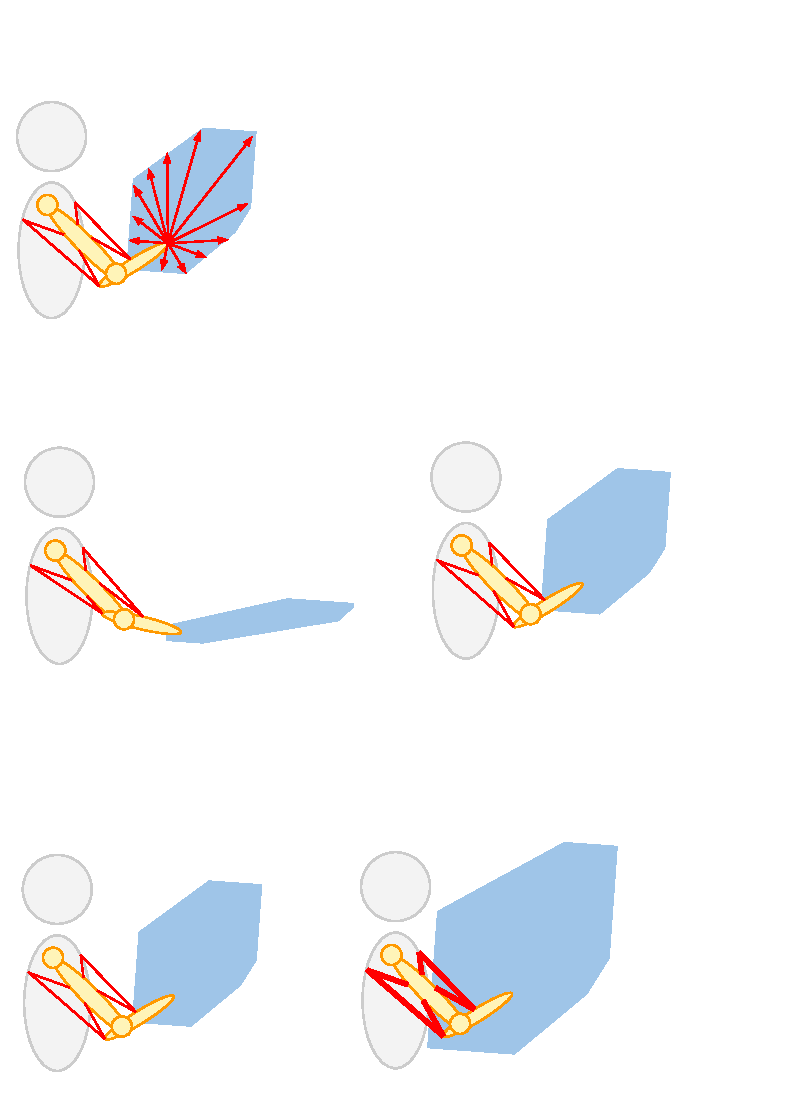
\includegraphics[trim={0 200 40 200},clip,width=0.7\linewidth]{img/chapter_1/ffs_characteristics.pdf}
    \caption{The force feasible sets of an individual vary according to a given posture.}
    \label{fig:ffs_posture}
\end{figure}


\begin{figure}[!htb]
    \captionsetup{justification=centering}
        \centering
        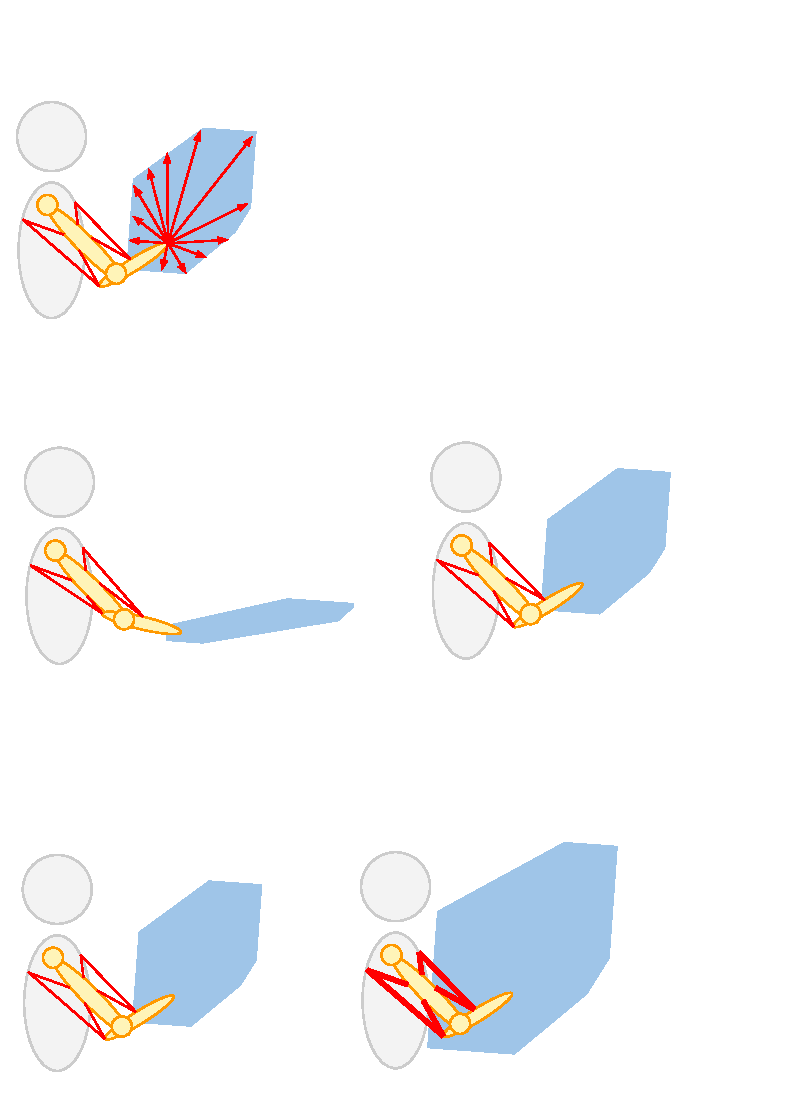
\includegraphics[trim={0 10 40 400},clip,width=0.7\linewidth]{img/chapter_1/ffs_characteristics.pdf}
    \caption{The force feasible sets of an individual vary depending on an individual's own physiology.}
    \label{fig:ffs_individual}
\end{figure}


Therefore, the set-theoretic perspective on force feasible sets offers significant potential, providing a concise way to convey to a robot biomechanical information about force boundaries producible in a human upper limb. Moreover, it allows leveraging the rich theoretical framework of modern mathematics to analyze and understand these sets, through various theoretical lenses (geometric, probabilistic, topological, etc.). Ultimately, a deeper understanding of force feasible sets can enhance the design and control of collaborative robots that interact effectively and safely with humans.

To explore this potential, this thesis will investigate the value of this set-theoretic approach in the context of personalizing musculoskeletal models in order to bring an answer to the following biomechanical challenge:

\begin{mdframed}
    \begin{center}
        \textbf{Challenge 3:} \\
        How can a set-theoretic approach to maximal isometric forces be used to quantitatively characterize muscle tension interactions
    \end{center}
\end{mdframed}

\section*{Thesis overview}
\addcontentsline{toc}{section}{Thesis overview}
This thesis involves the simulation of force feasible sets produced at the hand in a human upper-limb and their \emph{in vivo} counterparts. The different chapters contribute to a single objective: personalizing force feasible sets to an individual from maximal isometric force measurements in various postures. These chapters form a cohesive argument for this personalization process, creating a bridge between force feasible set modeling and biomechanical assumptions.

Chapter \ref{chapter:1} details how to derive force feasible sets, both \emph{in silico} and \emph{in vivo}, and examines the coherence between current modeling approaches and experimental measurements. Given the inherent set-theoretic nature of these representations, this chapter also explores current sensitivity analyses in biomechanics and considers more appropriate set-theoretic methods to assess how inter-individual muscle variability manifests in a set form.

Chapter \ref{chapter:2} delves into the computational challenges associated with the exact construction of a \emph{force polytope}, a force feasible set modeled under the assumption that muscle tensions are independent from each other. This construction necessitates computing either the vertices or the faces of a \emph{torque zonotope} representing all maximal joint torques generated by muscle tensions. The chapter introduces a novel vertex enumeration technique based on a specific selection of edges from a high-dimensional hypercube. This algorithm exhibits theoretical efficiency, with a time complexity comparable to the state-of-the-art. However, despite its efficiency, the inherent combinatorial complexity of vertex enumeration limits the applicability of this exact algorithm when the number of muscles exceeds a low amount ($>8$). Consequently, approximation alternatives are proposed for subsequent analyses in the thesis.

Chapter \ref{chapter:3} focuses on the theoretical implications of considering a high number of muscles in \emph{in silico} force feasible sets. This consideration is crucial because a force feasible set, by definition, reflects the combined action of all considered muscles, and its characteristics (volume, shape) are inherently dependent on the number of muscles included in the model. Simpler musculoskeletal models of the human upper limb may therefore fail to accurately capture experimentally observed force capacities. However, as demonstrated in the preceding chapter, increasing the complexity of the musculoskeletal model also increases the difficulty of modeling force feasible sets. To address this, the chapter draws upon established mathematical results from the \emph{Local Theory of Banach Spaces}, which investigates infinite-dimensional normed vector spaces through the lens of finite-dimensional ones, effectively bridging the gap between simplified models (seen as finite-dimensional spaces) and the complexities of real biological systems (represented as high-dimensional spaces). By applying these theoretical results to force feasible set modeling, the chapter argues that when a large number of muscles is considered, the \emph{size} (or \emph{scale}) of a force feasible set becomes the \emph{only} property influenced by muscle interactions. It demonstrates that any (convex) muscle interaction model induces force feasible sets which have the same ellipsoidal shape but with a size depending on the choice of the model. This scaling coefficient, termed the \emph{projection constant}, is explicitly computable for force polytopes and approximable for other tension models, enabling the construction of an ellipsoid approximation of a force polytope without resorting to computationally expensive combinatorial calculations. In other words, this chapter complexifies a musculoskeletal model in order to retrieve a simpler force feasible set representation as an ellipsoid.

Chapter \ref{chapter:4} focuses on quantifying the practical relevance of a set-theoretic approach to represent maximal isometric forces. We employ an optimization process to retrieve muscle parameterization in a 50-muscle musculoskeletal model (\cite{holzbaurModelUpperExtremity2005}), aiming to reproduce the default Holzbaur et al. force feasible sets in specific postures. Our methodology involves a careful analysis of the optimization results, considering factors such as different solving methods, posture sets, search-space sizes, parameters to be optimized, and force feasible set representations. Analyzing the solutions, the convergence of the algorithms, and their results for both polytopic and ellipsoidal force feasible set representations addresses the following questions:
\begin{enumerate}
    \item {\emph{Are 50 muscles sufficient to represent force feasible sets as ellipsoids?} The results suggest this is the case, as the generated force polytopes and their ellipsoid approximations yielded solutions with similar characteristics across almost all conditions in the optimization processes. This finding provides a practical lower bound on the number of muscles required for this approximation, supporting the theoretical results of the previous chapter, which indicated that the approximation holds in sufficiently \emph{high} dimensions;}
    \item {\emph{Is a set-theoretic approach relevant in musculoskeletal muscle personalization?} This analysis reveals that personalizing muscle parameters from force feasible sets in a real-world context is inherently challenging. While feasible in simpler cases with near-known solutions, the set-theoretic approach encounters significantly greater challenges in more complex scenarios. This difficulty is quantified through a novel index termed the \emph{enlargement ratio}, which relates the computational limitations of force polytope construction to the personalization process. By accounting for computational demands, we can assess the effectiveness of the personalization process and gain insights into the general difficulty of muscle personalization; }
    \item {\emph{Which muscle parameters most influence the force feasible set characteristics?} The results indicate a greater sensitivity to force-generating parameters compared to muscle geometry. Therefore, any such personalization process should prioritize the optimization of force-generating parameters.}
\end{enumerate}
These three findings directly inform the personalization process with \emph{in vivo} data in the next chapter.

Chapter \ref{chapter:5} integrates \emph{in silico} and \emph{in vivo} force feasible sets to generate personalized force capacities. An experimental protocol was conducted to collect maximal isometric force exertions at the hand in 26 directions and 4 postures from 10 participants. An upper-limb musculoskeletal model was then scaled to each participant. Building on Chapters \ref{chapter:3} and \ref{chapter:4}, which demonstrate the ellipsoidal nature of force polytopes, we utilize this approximation.  Furthermore, given the findings in Chapter \ref{chapter:4} regarding the limited influence of muscle geometry, we focus solely on adapting force-generating muscle properties. Also, Chapter \ref{chapter:2} highlighted that muscle tension interactions can be represented as a transformation of a sphere, providing a geometric interpretation for the ellipsoidal resemblance of force polytopes. This implies that individual muscle tension limits do not exert independent influence; rather, the average maximal tension across muscles primarily affects the scaling of a force feasible set. Consequently, only one parameter per posture require adjustment to align \emph{in silico} force feasible sets with \emph{in vivo} measurements. We apply this personalization process to the experimental data and evaluate the consistency of the theoretical results with empirical observations.

Finally, the Conclusion chapter will offer some closing remarks on this set-theoretic approach of maximal isometric forces, and draw the newest perspectives opened by the results found in this thesis. 

\section*{List of publications}
\addcontentsline{toc}{section}{List of publications}
During the thesis, two short publications were submitted and accepted. They are mentionned in Chapter \ref{chapter:4}, which focuses on muscle information extractable from force feasible sets. However, the work in these papers was preliminary to the work presented in Chapter \ref{chapter:4} and offered the first perspectives on the formulation of a muscle personalization process based on force feasible sets. The chapter serves as a more comprehensive exploration of these concepts, with a greater emphasis on the challenges of personalizing a musculoskeletal model, which neither paper addressed.

\begin{itemize}
    \item {G. Laisné, J-M. Salotti, and N. Rezzoug. ``Genetic Algorithms for Force Polytopes Prediction''. In: \emph{Computer Methods in Biomechanics and Biomedical Engineering} 26.sup1 (Oct. 2023), pp. 218-220.}
    \item {G. Laisné, J-M. Salotti, and N. Rezzoug. ``Derivative-Free Optimization Approaches for Force Polytopes Prediction''. In: \emph{ESANN 2023 - European Symposium on Artificial Neural Networks, Computational Intelligence and Machine Learning.} Bruges, Belgium, Oct. 2023, pp. 339-344.}
\end{itemize}

\section*{Notations}
\addcontentsline{toc}{section}{Notations}
This thesis employs a variety of mathematical objects, including vectors, matrices, lines, and sets, which are subject to manipulation and representation through diverse notational conventions. An example is the representation of a linear transformation between vector spaces by a matrix. While the notation may remain consistent, the context may necessitate an emphasis on either the matrix itself or the underlying linear transformation it encodes. This section serves to clarify the notational conventions for the objects employed in this thesis.

\begin{itemize}
    \item {\textbf{Common sets of numbers}: in uppercase and blackboard font. Examples: natural numbers $\mathbb{N}$, real numbers $\mathbb{R}$, strictly positive real number $\IR_{>0}$;}
    \item {\textbf{Bounded convex sets}: in uppercase, italic and caligraphic. Examples: cube $\mathcal{C}$, sphere $\mathcal{S}$, ellipsoid $\mathcal{E}$, polytope $\mathcal{P}$, zonotope $\mathcal{Z}$, orthotope $\mathcal{O}$;}
    \item{\textbf{Spaces}: in uppercase, italic letters. Examples: line $L$, plane $P$, hyperplane $H$, vector space $V$, Banach space $X$;}
    \item {\textbf{Coefficients}: in lowercase, italic and greek. Examples: $\lambda,\, \alpha,\, \mu \in\mathbb{R}$;}
    \item {\textbf{Points, integers and real numbers}: in lowercase, italic and latin. Examples: the points $p,\, q,\, r \in E$, the integers $n,\,m\in\mathbb{N}$ and the real $x\in \mathbb{R}$;}
    \item {\textbf{Vectors}: in lowercase, bold and latin. Vectors can be indexed by non-bold characters when needed. Examples: $\mathbf{x},\, \mathbf{y},\, \mathbf{q} \in \mathbb{R}^n$ and $\mathbf{x} = (x_1,\, \dots,\, x_n)$;}
    \item {\textbf{Matrices}: in uppercase, italic and block letters. Example: $M \in \mathbb{R}^{n\times m}$;}
    \item {\textbf{Functions}: in lowercase, italic and in latin or greek, with parentheses. Examples: the function $f\colon \mathbb{R}\rightarrow \mathbb{R}$ such that $f(x) = x^3$;}
    \item {\textbf{Affine maps}: An affine map denotes a linear mapping followed by a translation. The linear part can be represented by a matrix, and the translation by a vector. For instance, the linear transformation of a vector $\mathbf{x}\in\IR^3$ through $A \in \IR^{3\times 3}$, then translated by $\mathbf{t}\in\IR^3$, is noted $A\mathbf{x} + \mathbf{t}$. This notation is particularly useful for sets, where for instance the affine transformation of the 3D cube $\mathcal{C}=[0,1]^3$ under the same conditions is simply noted $A\mathcal{C} + \mathbf{t}$.}
\end{itemize}
